\documentclass[12pt]{article}
\usepackage{amsmath}
\usepackage{amssymb}
\usepackage[letterpaper,margin=0.85in,centering]{geometry}
\usepackage{fancyhdr}
\usepackage{enumerate}
\usepackage{lastpage}
\usepackage{multicol}
\usepackage{graphicx}

\reversemarginpar

\pagestyle{fancy}
\cfoot{Page \thepage \ of \pageref{LastPage}}\rfoot{{\bf Total Points: 60}}
\chead{MATH 2580A}\lhead{Test \#1}\rhead{Thursday, 11\textsuperscript{th} February, 2015}

\newcommand{\points}[1]{\marginpar{\hspace{24pt}[#1]}}
\newcommand{\skipline}{\vspace{12pt}}
%\renewcommand{\headrulewidth}{0in}
\headheight 30pt

\newcommand{\di}{\displaystyle}
\newcommand{\R}{\mathbb{R}}
\newcommand{\N}{\mathbb{N}}
\newcommand{\Z}{\mathbb{Z}}
\newcommand{\pd}[2]{\dfrac{\partial #1}{\partial #2}}
\newcommand{\rd}[2]{\dfrac{d #1}{d #2}}
\newcommand{\dotp}{\boldsymbol{\cdot}}

\begin{document}

\author{Instructor: Sean Fitzpatrick}
\thispagestyle{plain}
\begin{center}
\emph{University of Lethbridge}\\
Department of Mathematics and Computer Science\\
11\textsuperscript{th} February, 2016, 1:40 - 2:55 pm\\
{\bf Math 2580A - Term Test \#1}\\
\end{center}
\skipline \skipline \skipline \noindent \skipline
Last Name:\underline{\hspace{350pt}}\\
\skipline
First Name:\underline{\hspace{348pt}}\\
\skipline
Student Number:\underline{\hspace{322pt}}\\


\vspace{0.5in}


\begin{quote}
 Record your answers below each question in the space provided.    {\bf Left-hand pages may be used as scrap paper for rough work.}  If you want any work on the left-hand pages to be graded, please indicate so on the right-hand page.
 
 \bigskip
 
Partial credit will be awarded for partially correct work, so be sure to show your work, and include all necessary justifications needed to support your arguments. 

The value of each problem is indicated in the left-hand margins. The value of a problem does not always indicate the amount of work required to do the problem.

Outside aids, including, but not limited to, cheat sheets, smart phones, laptops, spy cameras, drones, and divine intervention, are not permitted. You can keep a calculator with you if it makes you feel better.
\end{quote}


\vspace{0.5in}

For grader's use only:

\begin{table}[hbt]
\begin{center}
\begin{tabular}{|l|r|} \hline
Page&Grade\\
\hline \hline
\cline{1-2} 2 & \enspace\enspace\enspace\enspace\enspace\enspace/6\\
\cline{1-2} 3 & \enspace\enspace\enspace\enspace\enspace\enspace/12\\
\cline{1-2} 4 & \enspace\enspace\enspace\enspace\enspace\enspace/12\\
\cline{1-2} 5 & \enspace\enspace\enspace\enspace\enspace\enspace/12\\
\cline{1-2} 6 & \enspace\enspace\enspace\enspace\enspace\enspace/12\\
\cline{1-2} 7 & \enspace\enspace\enspace\enspace\enspace\enspace/6\\
\cline{1-2} Total & \enspace\enspace\enspace\enspace\enspace\enspace/60\\
\hline
\end{tabular}

\skipline

\skipline

\skipline


\end{center}
\end{table}
\newpage


\begin{enumerate}
\item Match the following functions with (a) its graph, and (b) its contour plot. (Write the letter ($f$, $g$, or $h$) corresponding to the function next to the correct graph and contour plot.)\points{6}
\[
 \quad f(x,y) = \sin x-\sin y \quad g(x,y) = \sin(x-y) \quad h(x,y) = e^x\cos y 
\]
Hint: think about the curves you obtain from each function by holding either $x$ or $y$ constant.

\begin{multicols}{2}
 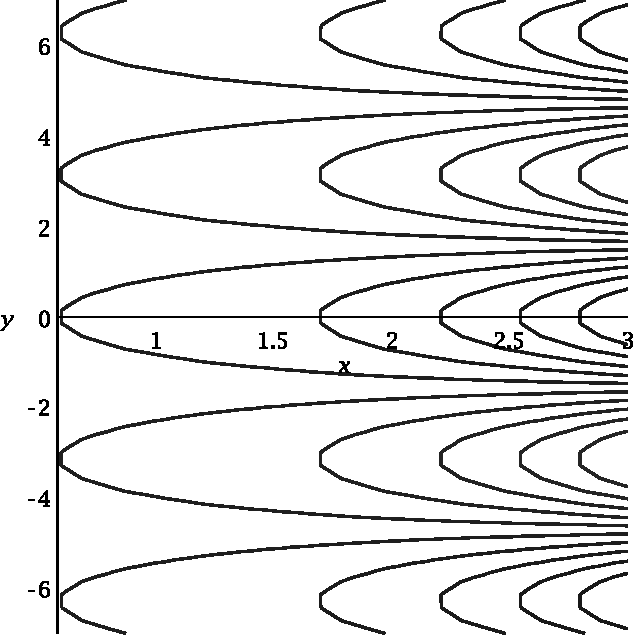
\includegraphics[width=2in]{T1ccont}

 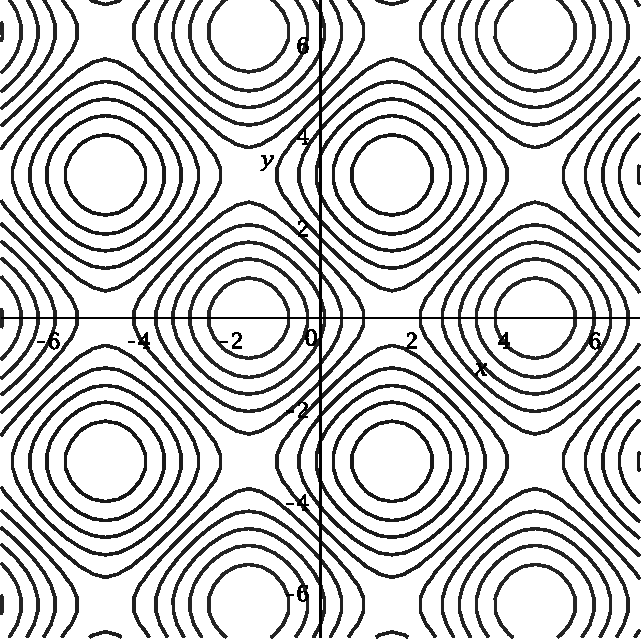
\includegraphics[width=2in]{T1dcont}

 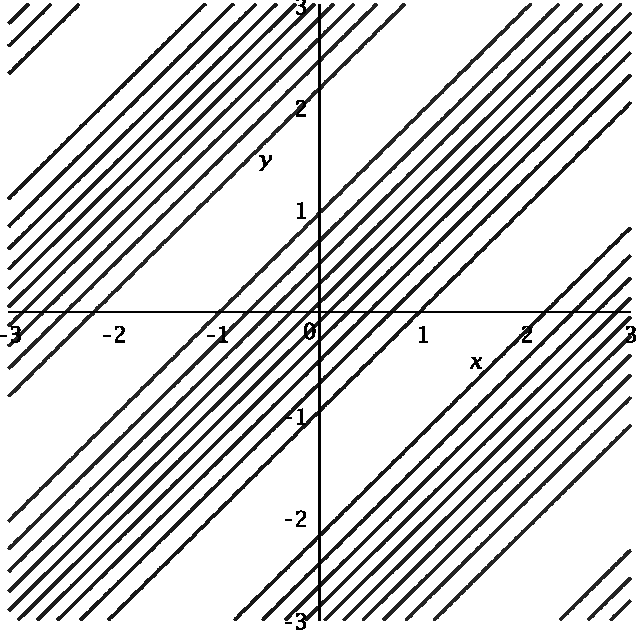
\includegraphics[width=2in]{T1bcont}

\columnbreak

 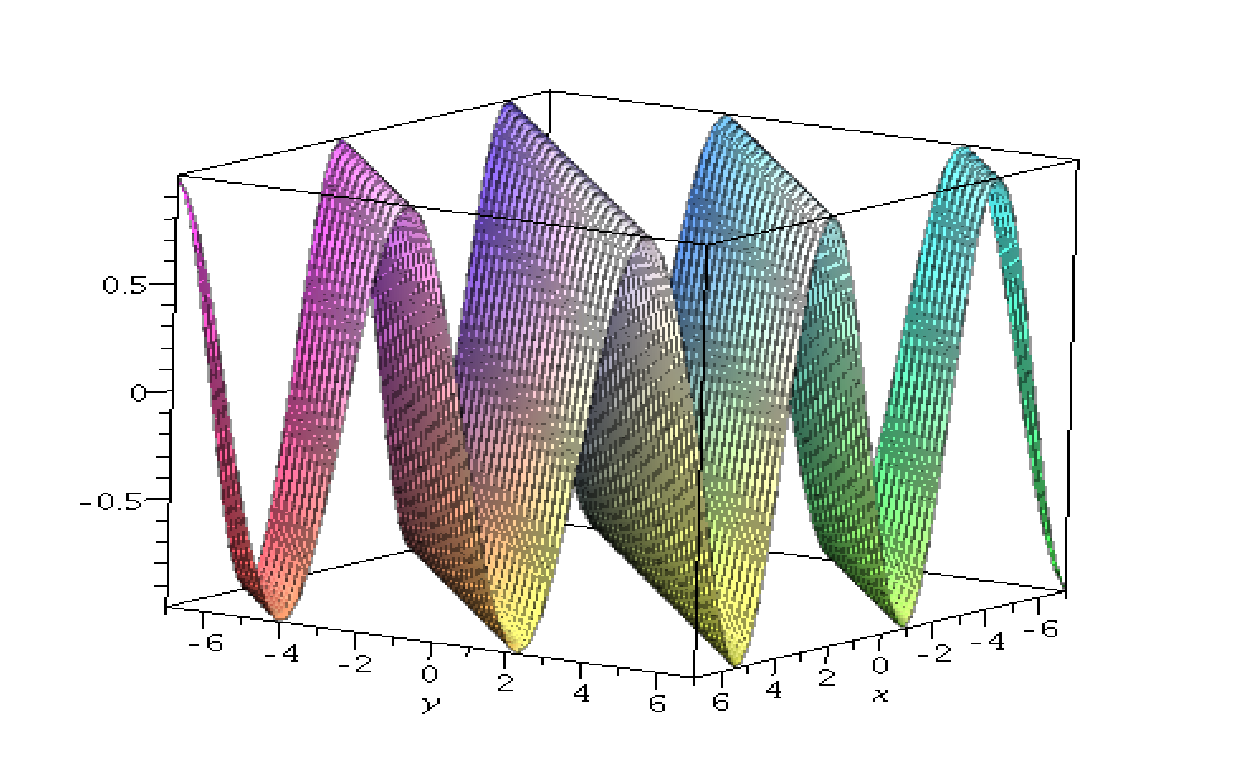
\includegraphics[width=3in]{T1bsurf}

 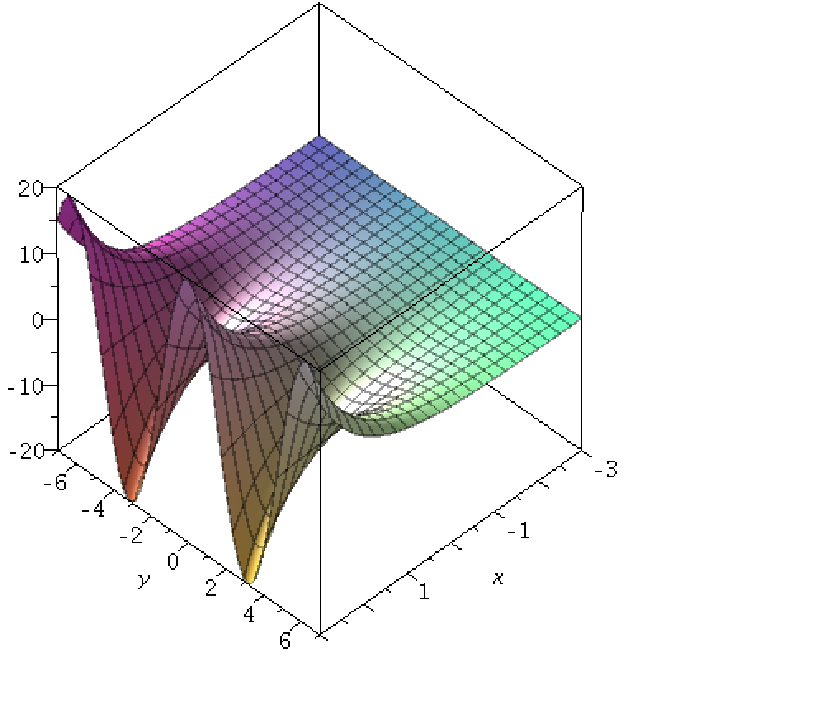
\includegraphics[width=3in]{T1csurf}

 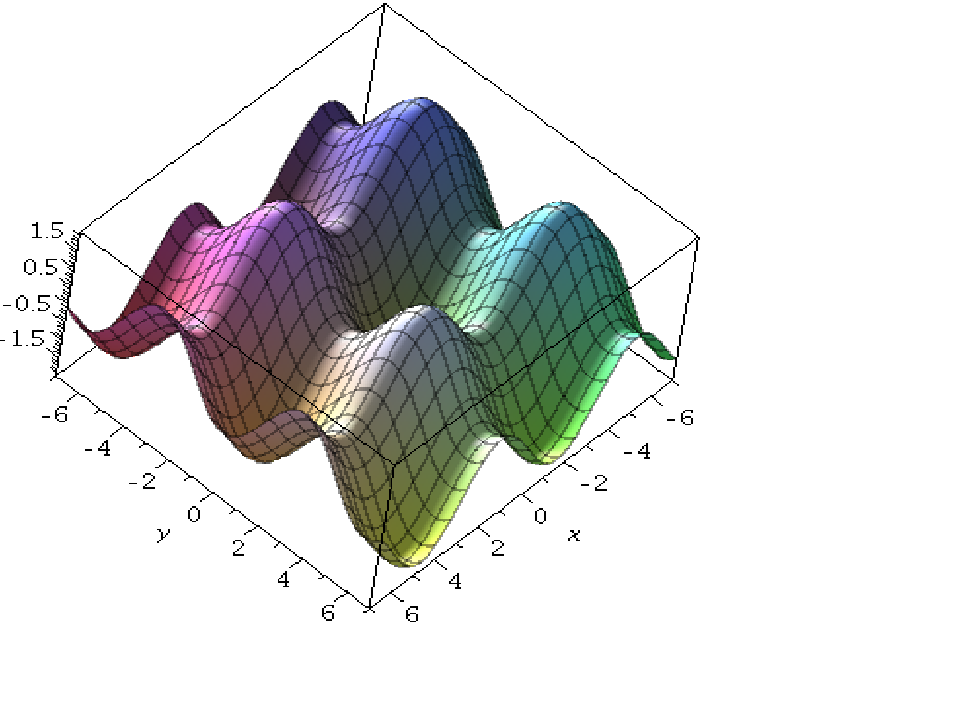
\includegraphics[width=3in]{T1dsurf}
\end{multicols}

\newpage

\item Consider the function $f(x,y) = 3\sqrt{x^2+y^3}$.
\begin{enumerate}
 \item Calculate the partial derivatives $f_x$ and $f_y$.\points{4}

\vspace{2in}

 \item Find the equation of the tangent plane to the graph $z=3\sqrt{x^2+y^3}$ at the point $(1,2,9)$. \points{4}

\vspace{3in}

 \item Approximate the value of $3\sqrt{(0.99)^2+(2.02)^3}$. \points{4}

\end{enumerate}
\newpage

\item Show that $\di \lim_{(x,y)\to (0,0)}\frac{xy}{x^2+y^2}$ does not exist. \points{4}

\vspace{3in}

\item Calculate the derivative of the function $f(x,y,z) = 2xy^2-3x^2z+4xyz$ at the point $(2,1,-1)$ in the direction of the vector $\vec{v} = \langle \frac{2}{3}, \frac{1}{3}, \frac{-2}{3}\rangle$. \points{8}

\newpage

\item Calculate $\pd{z}{u}$ and $\pd{z}{v}$, where $z = x^2y-2xy^2$, if $x=2uv^2$, and $y=4u^2v$, using the Chain Rule. \points{8}

\vspace{4in}

\item Find the equation of the tangent plane to the surface $xy^2+yz^2+xyz=5$ at the point $(2,1,1)$. \points{4}

\newpage



\item Find and classify the critical points of the function $f(x,y)=2x^3+y^3-3x^2-3y$.\points{12}

\newpage


\item Recall that a function $f:D\subseteq \R^n\to \R$ is differentiable at $\vec{a}\in \R^n$ if and only if
\begin{equation*}
\lim_{\vec{x}\rightarrow \vec{a}}\frac{\lvert f(\vec{x})-f(\vec{a}) - \nabla f(\vec{a})\cdot (\vec{x}-\vec{a})\rvert}{||\vec{x}-\vec{a}||} = 0.
\end{equation*}
Using this definition, prove that if $f$ is differentiable at $\vec{a}$, then for any unit vector $\vec{v}$,\points{6}
\[
 \lim_{h\to 0}\frac{f(\vec{a}+h\vec{v})-f(\vec{a})}{h} = \nabla f(\vec{a})\dotp \vec{v}.
\]
(In other words, use the definition of differentiability to derive the gradient formula for the directional derivative.)\\
{\em Hint:} If the limit in the definition above exists, you use any path along which $\vec{x}$ approaches $\vec{a}$ to evaluate it.
\end{enumerate}
\newpage

\begin{center}
List of potentially useful formulas and facts:
\end{center}


\begin{itemize}

\item Clairaut's Theorem: If $f$ is defined on a disk $D$ and $f_{xy},\, f_{yx}$ are continuous on $D$, then $f_{xy}=f_{yx}$ on $D$.
\item The linearization of a function $f(x,y)$ at a point $(a,b)$ is given by
\[
L(x,y) = f(a,b)+f_x(a,b)(x-a)+f_y(a,b)(y-b),
\]
and the equation of the tangent plane to $z=f(x,y)$ at the point $(a,b,f(a,b))$ is $z=L(x,y)$.
\item If the first order partial derivatives of a function $f$ exist in a neighborhood of a point, and are continuous at that point, then $f$ is differentiable at that point.
\item If $w=f(x,y,z)$ and $x=x(t),\, y=y(t),\, z=z(t)$, then
\[
\frac{dw}{dt} = \pd{f}{x}\rd{x}{t}+\pd{f}{y}\rd{y}{t}+\pd{f}{z}\rd{z}{t}.
\]
If $x=x(u,v), \, y=(u,v),\, z=z(u,v)$, then
\[
\pd{w}{u} = \pd{f}{x}\pd{x}{u}+\pd{f}{y}\pd{y}{u}+\pd{f}{z}\pd{z}{u},
\]
with a similar formula for $\partial w/\partial v$, and variations on the above Chain Rule formulas for other numbers of variables.
\item The derivative of $f$ in the direction of a vector $\mathbf{v}$ at a point $\mathbf{x}_0$ can be computed according to $\di d_{\mathbf{v}}f(\mathbf{x}_0) = \frac{\nabla f(\mathbf{x}_0)\dotp \mathbf{v}}{\lVert\mathbf{v}\rVert}$.
\item The tangent plane to a level surface $f(x,y,z)=k$ at a point $(a,b,c)$ is given by \\$\nabla f(a,b,c)\dotp\langle x-a, y-b, z-c\rangle = 0$.
\item The tangent vector to a curve $\mathbf{r}(t) = \langle x(t),y(t),z(t)\rangle$ is $\mathbf{r}'(t) = \langle x'(t), y'(t), z'(t)\rangle$.
\item Suppose $f$ has a critical point at $(a,b)$, and the second derivatives of $f$ are continuous on a neighborhood of $(a,b)$. Let $D = f_{xx}(a,b)f_{yy}(a,b)-f_{xy}(a,b)^2$. If
\begin{enumerate}[(a)]
\item $D>0$ and $f_{xx}(a,b)>0$, then $f$ has a local minimum at $(a,b)$.
\item $D>0$ and $f_{xx}(a,b)<0$, then $f$ has a local maximum at $(a,b)$.
\item $D<0$, then $f$ has a saddle point at $(a,b)$.
\end{enumerate}

\end{itemize}


\end{document}